\chapter{Sistema di coordinazione}\label{cap:sistema-coordinazione}

\section{Scopo del sistema}
Il sistema di coordinazione è il componente che si occupa di gestire i lampioni, regolandone l'accensione e lo spegnimento in base alle informazioni che ha a disposizione.\\

Tramite algoritmi sofisticati, il sistema di coordinazione è in grado di gestire l'illuminazione in modo efficiente.

\subsection{Requisiti coperti dal sistema}

\subsubsection{RF\_05}

RF\_05: Il sistema deve accendere un'area per un lasso di tempo preconfigurato quando rileva persone in prossimità dello stesso.

\subsubsection{RF\_06}

RF\_06: Il sistema deve riportare l'intensità luminosa dell'area al valore di default una volta passato il tempo impostato.

\subsubsection{RF\_19}

RF\_19: Il sistema deve essere in grado di ricevere informazioni dal sensore in modalità push.

\section{Descrizione del sistema}

Il sistema utilizza molteplici paradigmi. L'architettura generale è di tipo esagonale.

Il programma eseguirà azioni quando attivato da eventi esterni, quali l'arrivo di un nuovo stato da mqtt oppure l'arrivo di una richiesta da parte dell'utente collegato alla webapp\footnote{Vedi sezione \ref{cap:webapp}}.

Le componenti principali saranno:

\begin{itemize}
    \item \textbf{Porta ricevente MQTT}: si occupa di ricevere i messaggi da MQTT e di inoltrarli al sistema ad eventi;
    \item \textbf{Interfaccia REST}: si occupa di ricevere le richieste degli utenti e di inoltrarle al sistema ad eventi;
    \item \textbf{Pila di payload}: É una pila contenente i payload di dati da analizzare;
    \item \textbf{Algoritmo di analisi}: Dato un payload si occupa di analizzarlo e di generare un nuovo stato;
\end{itemize}

La pila di Payload usa il paradigma del \textbf{Producer-Consumer}, in cui il produttore è la porta ricevente, mentre il consumatore è l'algoritmo di analisi.

É poi presente un database\footnote{Vedi sezione relativo al database e alla sua progettazione \ref{cap:db-sistema-coordinatore}} al quale il sistema si connette, per mantenere gli stati anche in caso di reboot del sistema.

Inoltre, se il programma farà comunque del caching dei dati, sarà comunque nel database che verranno depositati i dati quando la cache diventa troppo grande.

\section{Architettura del sistema}

Il sistema è composto da un'interfaccia rest, un'interfaccia mqtt, un collegamento ad un db e un algoritmo di analisi.

\subsection{Entità del sistema}

\begin{itemize}
    \item \textbf{AreaAnagrafica}: Contiene le informazioni relative ad un'area, quali la posizione, il nome, il tipo di illuminazione, ecc.
    \item \textbf{LampAnagrafica}: Contiene le informazioni relative ad un lampione, quali la posizione, il nome, il tipo di illuminazione, ecc.
    \item \textbf{Misuratore}:
    \item \textbf{SensoreAnagrafica}: Contiene le informazioni relative ad un sensore, quali la posizione, il nome, il tipo di sensore, ecc.
\end{itemize}

\subsection{Classi legate al database}

Il database viene gestito come repository, e ognuna delle entità viene gestita come tale.

Le classi relative ai repository sono:

\begin{itemize}
    \item \textbf{AreaRepository}: Fornisce l'accesso al database per le aree;
    \item \textbf{LampRepository}: Fornisce l'accesso al database per i lampioni;
    \item \textbf{MisuratoreRepository}: 
    \item \textbf{SensoreRepository}: Fornisce l'accesso al database per i sensori;
\end{itemize}

Le classi sopra descritte sono visibili in figura \ref{fig:coordinazione_db}

\begin{figure}[h]
    \centering
    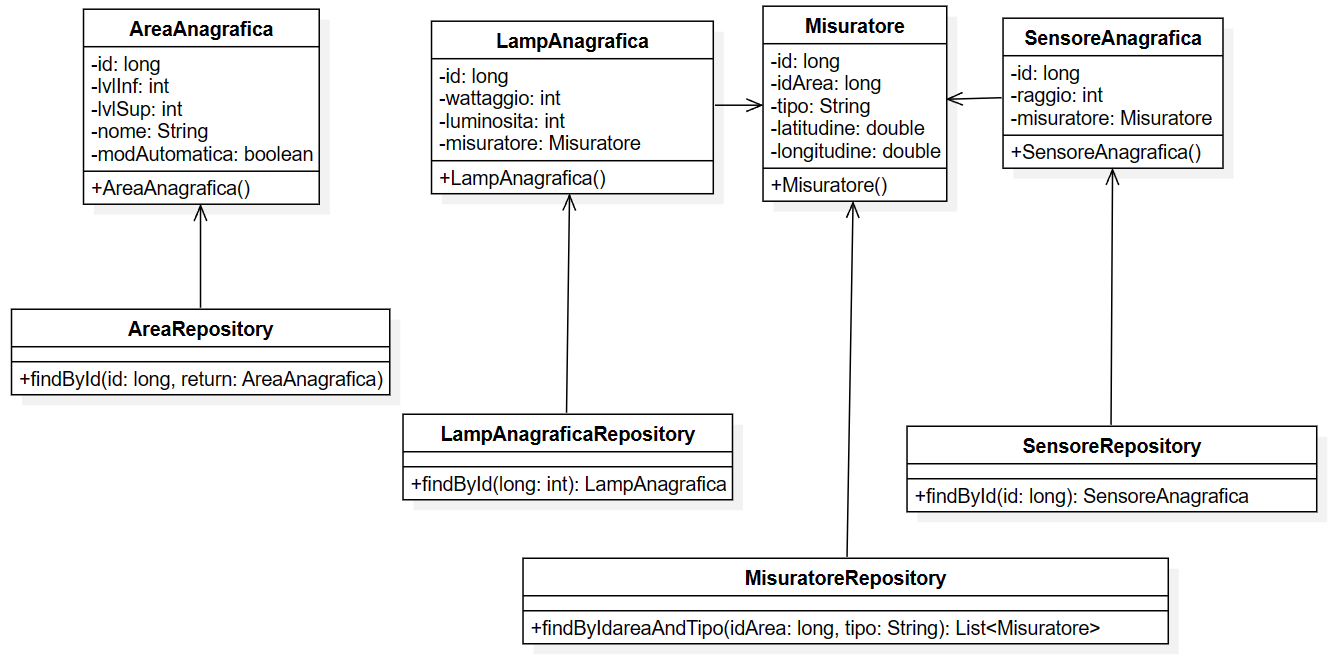
\includegraphics[width=\textwidth]{img/illuminazione_repository.png}
    \caption{Diagramma delle classi relative ai repository e al sistema connesso al database}
    \label{fig:coordinazione_db}
\end{figure}

Queste classi effettuano le operazioni sul db tramite JPA.

\subsection{Classi di configurazione}

La classe \textbf{Beanconfig} contiene tutti i bean di Spring relativi alla configurazione per mqtt e per il database.

\subsection{Classi legate ad MQTT}

Per la gestione di mqtt sono presenti le seguenti classi visibili in figura \ref{fig:coordinazione_mqtt}

\begin{figure}[h]
    \centering
    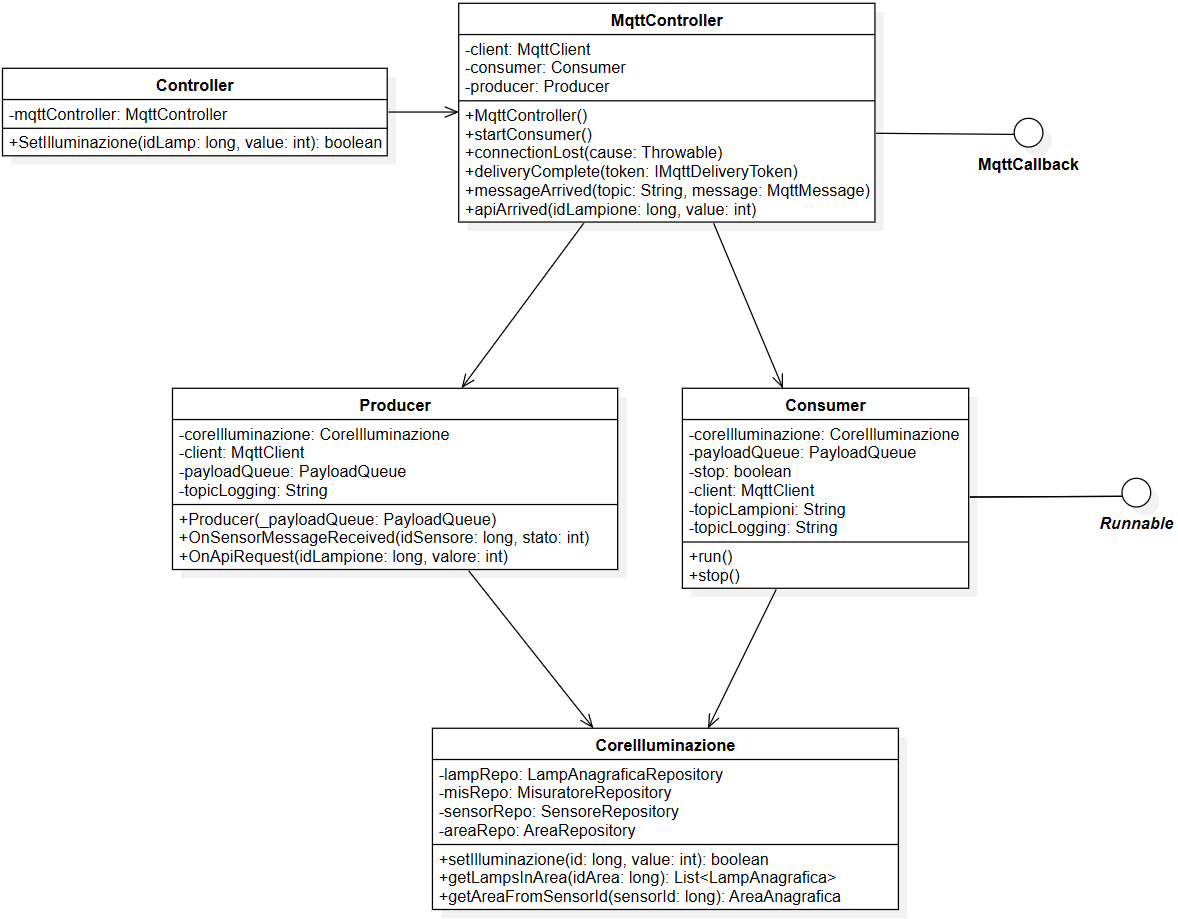
\includegraphics[width=\textwidth]{img/illuminazione_mqtt.png}
    \caption{Diagramma delle classi relative alla parte mqtt del sistema di coordinazione}
    \label{fig:coordinazione_mqtt}
\end{figure}


\begin{itemize}
    \item \textbf{MqttController}: Si occupa di gestire la ricezione dei messaggi da mqtt e di inoltrarli al sistema ad eventi;
    \item \textbf{Producer}: Questa classe rimane in ascolto delle rilavazioni mqtt, quando dal topic sensore arriva un cambiamento, questo viene segnalato al logging\footnote{Il logging poi loggerà l'informazione}. In ultimo genera un payload e lo aggiunge alla coda dei payload da processare;
    \item \textbf{Consumer}: Quando vede che la coda dei payload non è vuota raccoglie le operazioni da fare, analizza lo stato e modifica la luminosità dei lampioni via mqtt, inoltre aggiorna il database con il nuovo stato;
\end{itemize}

\subsubsection{Payloads}

I payloads sono un oggetto che contiene le informazioni necessarie per l'analisi e la modifica dello stato di illuminazione.

Queste classi vengono descritte nell'immagine \ref{fig:coordinazione_payload}.

\begin{figure}[h]
    \centering
    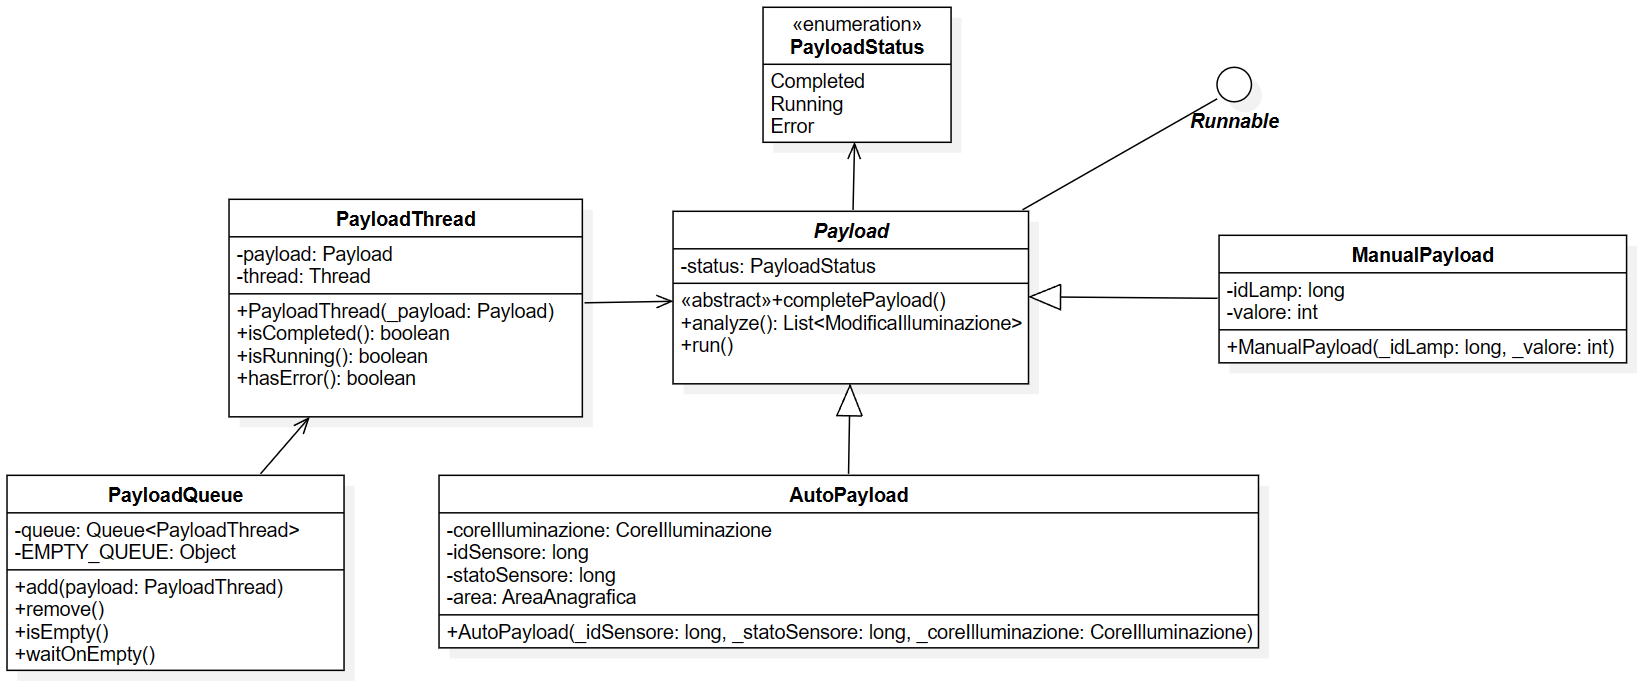
\includegraphics[width=\textwidth]{img/illuminazione_payload.png}
    \caption{Diagramma delle classi relativa ai payloads}
    \label{fig:coordinazione_payload}
\end{figure}

\paragraph{Payload} è un'interfaccia che contiene i metodi comuni a tutti i payloads.

\paragraph{PayloadQueue} è una coda di payload, che contiene i payload da processare.

\paragraph{PayloadThread} è un thread che si occupa di processare i payload.

\paragraph{PayloadStatus} è un enum che contiene i possibili stati dei payload.

\paragraph{PayloadManual} è un payload che contiene le informazioni per un'analisi manuale.

\paragraph{PayloadAuto} è un payload che contiene le informazioni per un'analisi automatica.

I payload manuali e automatici sono thread che fanno le loro operazioni in parallelo, controllano se c'è da modificare uno stato e in caso positivo preparano le informazioni per il consumer.
